\documentclass[10pt]{article}
\usepackage[margin=0.9in]{geometry}
\usepackage{graphicx,booktabs,float,longtable,xcolor}
\setlength{\parskip}{0.4em}\setlength{\parindent}{0pt}
\title{Hotel Schematic Proposal\\\large Program, planning-level layout, code screen and open questions}
\author{RNGD side project --- prototype output, not for construction}
\date{\today}
\begin{document}
\maketitle

\section{Summary}
Program: 117 guest keys in 21 rows, 59,350 SF net shared/BOH/guest area,
across six levels. Source gross area: 74,195 SF. Planning-level schematic: five upper levels of
double-loaded corridor, each with a core at the west end. The schematic fails two screens from RNGD's
own IBC rule set: six stories above grade (rule limit five) and a dead-end corridor of about
183 ft (limit 50 ft). These are design findings, not code determinations.

\section{Program}
\begin{longtable}{p{7.2cm}rrl}\toprule
Room type & Count & Area (SF) & Category \\ \midrule
\endhead
ADA Corner Suite & 1 & 852 & guest \\
ADA King Spa & 2 & 920 & guest \\
ADA QQ & 2 & 892 & guest \\
ADA Suite & 2 & 1,278 & guest \\
Corner Suite & 2 & 1,728 & guest \\
King & 69 & 23,692 & guest \\
King Spa & 3 & 1,379 & guest \\
QQ & 33 & 11,342 & guest \\
Suite & 3 & 1,920 & guest \\
Corridor & 1 & 1,335 & shared \\
Gym & 1 & 968 & shared \\
Lobby & 1 & 2,865 & shared \\
Restrooms (M/W) & 1 & 405 & shared \\
Luggage & 1 & 122 & shared \\
BOH / Bus & 1 & 1,718 & boh \\
Hotel Kitchen / Pantry & 1 & 331 & boh \\
BOH storage (BOH, Housekeeping, Janitor, Ice, IT, Supplies) & 1 & 1,611 & boh \\
Loading & 1 & 282 & boh \\
MEP Service & 1 & 309 & boh \\
Stairs & 1 & 1,868 & core \\
White Box Retail (tenant) & 1 & 3,533 & tenant \\
\bottomrule
\end{longtable}
Source: Project Renegade Living + Lodging Prototype, cover sheet (06/20/25). Guest-room areas are type averages (type total divided by count).
Source subtotals reconcile to 59,350 SF; the table sums to 59,350 SF because of one-square-foot rounding in the source.

\section{Gross area and net-to-gross}
\begin{tabular}{lr}\toprule
Level & Gross SF (source) \\ \midrule
Level 1 & 12,485 \\
Level 2 & 12,342 \\
Level 3 & 12,342 \\
Level 4 & 12,342 \\
Level 5 & 12,342 \\
Level 6 & 12,342 \\
\midrule Total & 74,195 \\ \bottomrule
\end{tabular}

Source ratio gross/net: 1.25. Meeting-derived rule (33\% circulation, 8\% wall burden, rounded up to 100 SF):
85,300 SF. These rules were stated in the kickoff meeting, not confirmed by RNGD, and are shown as a comparison only.

\section{Schematic}
Envelope: 170 x 265 ft (synthetic, pending the real lot). Each upper level is one double-loaded wing:
rooms on both sides of a 6-ft corridor, room depth 26 ft, width from the type area, core (two stairs and elevators) at the west end.
Guest-room types are placed in the order of area, so suites are spread across levels.

\begin{figure}[H]\centering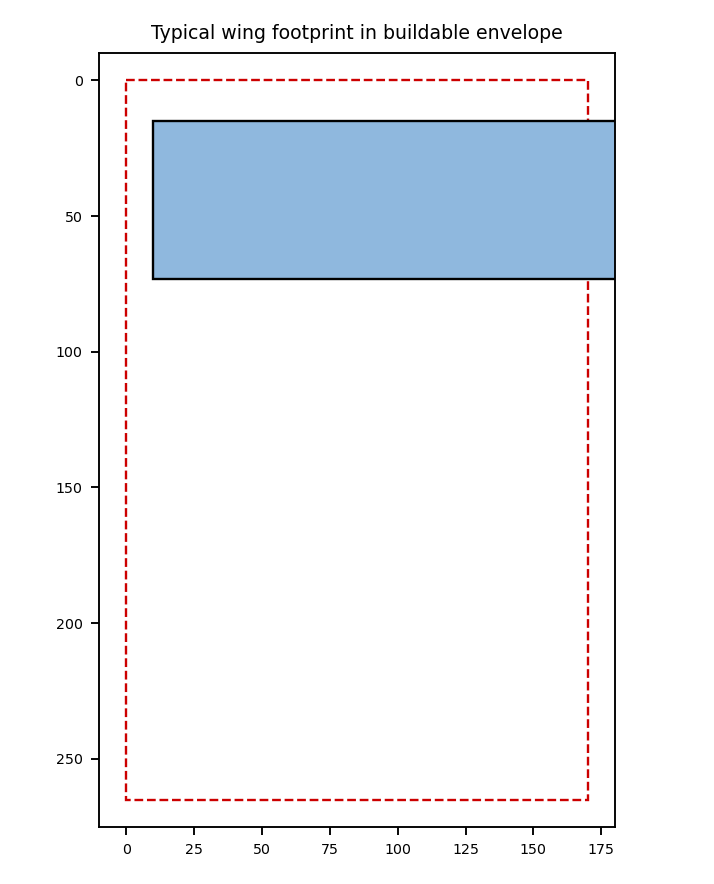
\includegraphics[width=0.45\linewidth]{site.png}\caption{Wing footprint in the buildable envelope.}\end{figure}
\begin{figure}[H]\centering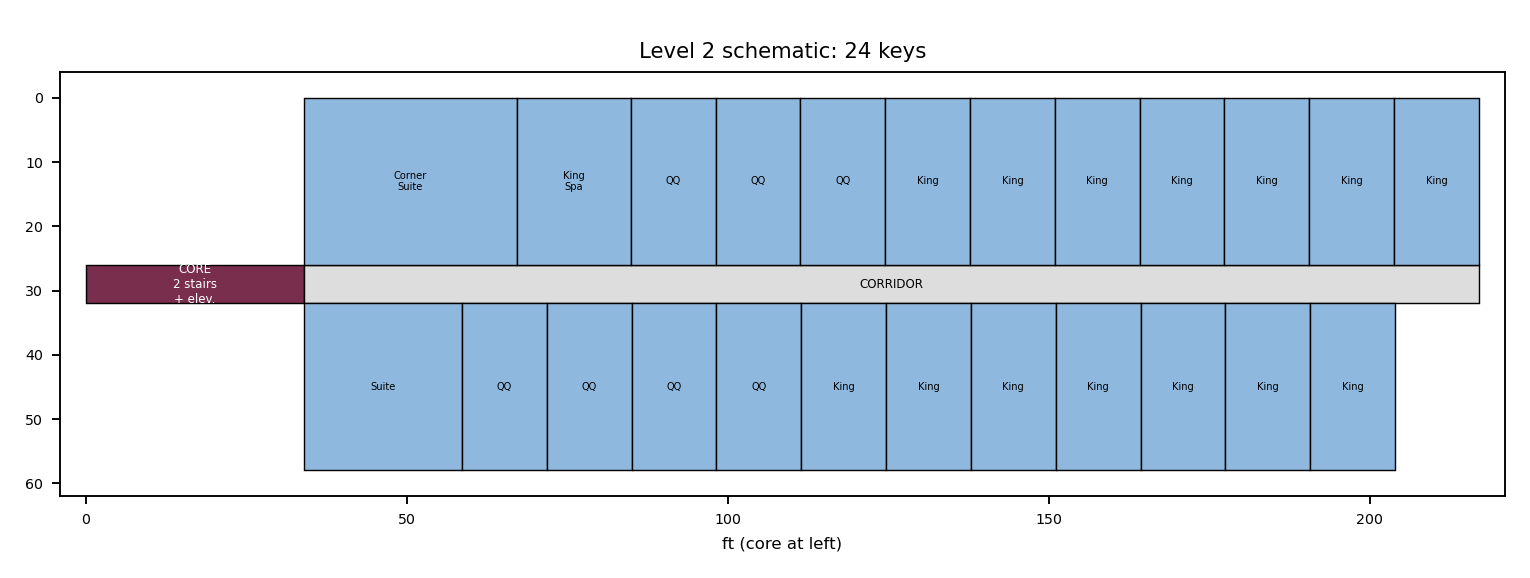
\includegraphics[width=\linewidth]{level_2.png}\caption{Level 2: 24 guest keys, wing 217 x 58 ft.}\end{figure}
\begin{figure}[H]\centering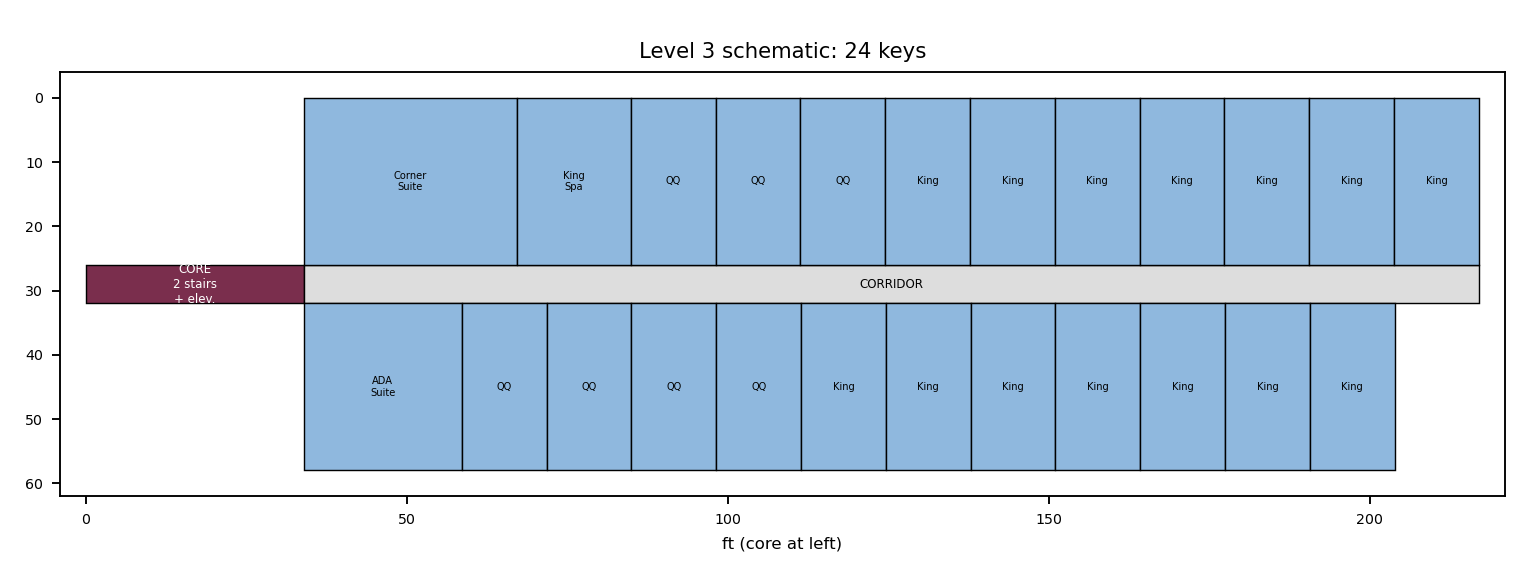
\includegraphics[width=\linewidth]{level_3.png}\caption{Level 3: 24 guest keys, wing 217 x 58 ft.}\end{figure}
\begin{figure}[H]\centering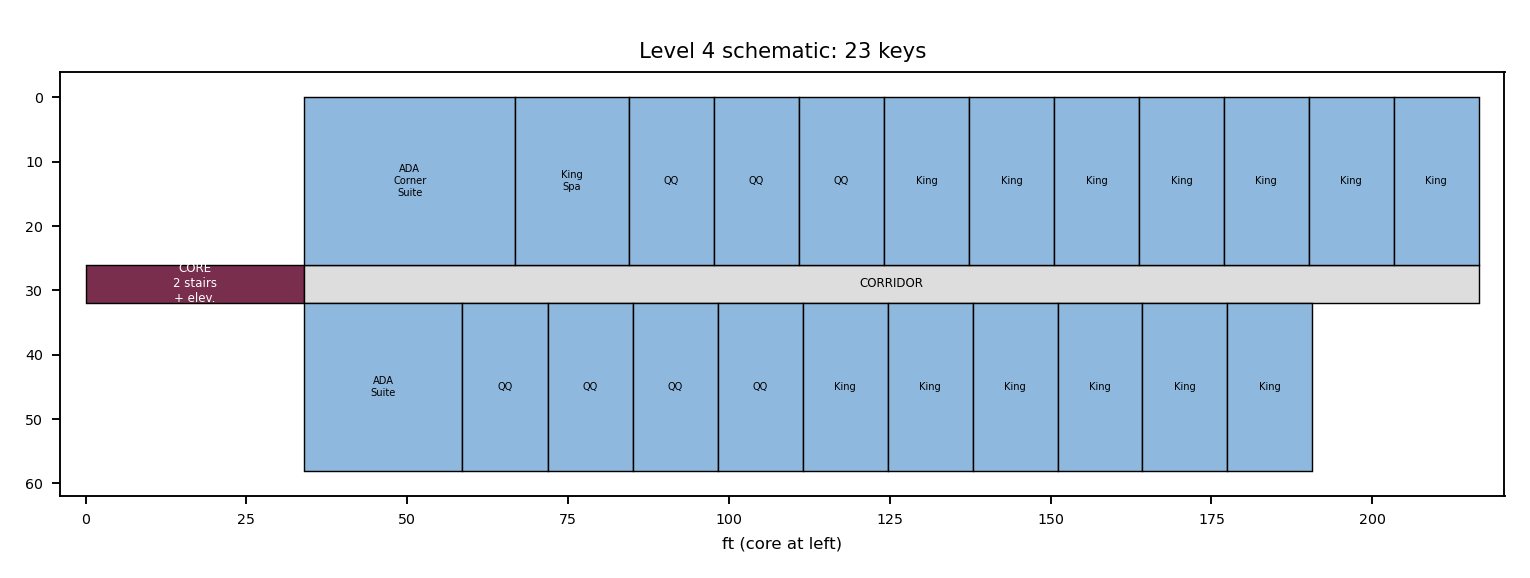
\includegraphics[width=\linewidth]{level_4.png}\caption{Level 4: 23 guest keys, wing 217 x 58 ft.}\end{figure}
\begin{figure}[H]\centering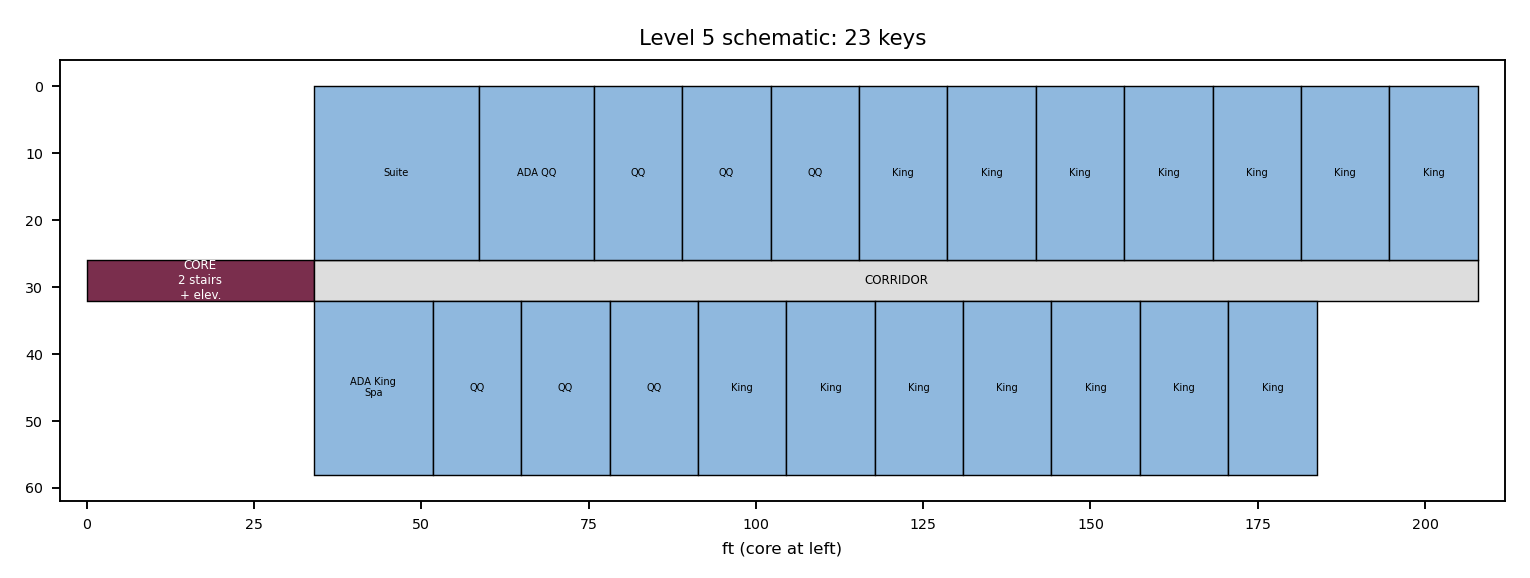
\includegraphics[width=\linewidth]{level_5.png}\caption{Level 5: 23 guest keys, wing 208 x 58 ft.}\end{figure}
\begin{figure}[H]\centering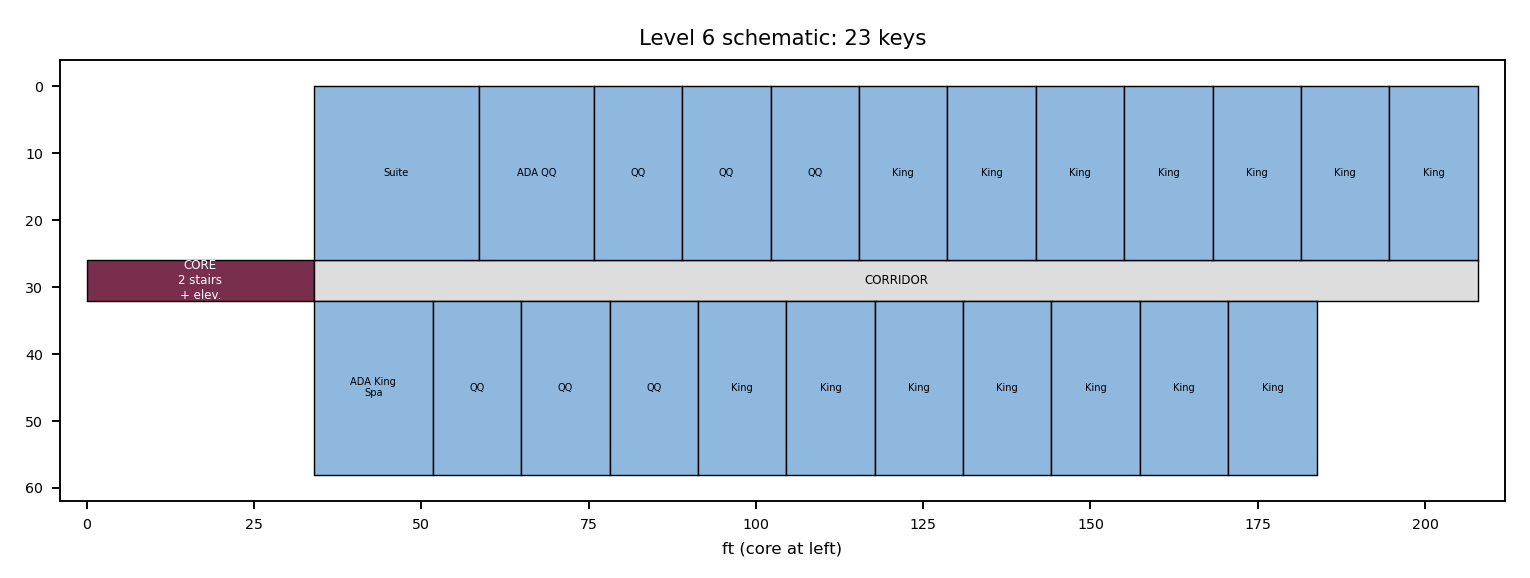
\includegraphics[width=\linewidth]{level_6.png}\caption{Level 6: 23 guest keys, wing 208 x 58 ft.}\end{figure}

\section{Code and program screen}
Checks use the IBC rule subset in RNGD's rule database (2021 IBC, Type IIA sprinklered R-1 hotel). The overall planning screen is not a code determination.
\begin{longtable}{p{4.2cm}p{4.6cm}p{3cm}l}\toprule
Check & Required & Provided & Status \\ \midrule
\endhead
Keys placed & 117 & 117 & PASS \\
Stories above grade & $\le$ 5 (IBC-R1-007, Type IIA sprinklered R-1) & 6 & FAIL \\
Building height (ft) & $\le$ 85 (IBC-R1-005, Type IIA) & 66.5 & PASS \\
Dead-end corridor (ft) & $\le$ 50 (IBC-R1-027) & 183 & FAIL \\
Exit travel distance (ft) & $\le$ 250 (IBC-R1-023) & 183 & PASS \\
Fits buildable envelope & 170 x 265 ft & 217 x 58 ft & PASS \\
\bottomrule
\end{longtable}

\section{Assumptions}
\begin{itemize}
\item Synthetic lot and envelope (170 x 265 ft). The real site and setbacks are not yet supplied.
\item Corridor double-loaded, 6 ft clear; room depth 26 ft; core 34 x 24 ft; two stairs per core.
\item Ground level shows program area only (no room layout). Parking is not modeled.
\item Accessible rooms, fire lane and fire access are not modeled. Code parameters from the R-1 rule set only.
\item Keys are split evenly across five upper levels in order of area.
\end{itemize}

\section{Open questions}
\begin{enumerate}
\item \textbf{Which area of the Level 1 and Level 2 drawing was meant?} The reference coordinate note
(scale 1.08 to original image) did not identify a room, stair or gridline. Please mark the spot.
\item Confirm circulation (33\%) and wall burden (8\%) percentages, or give RNGD's own factors.
\item Confirm the real lot geometry, setbacks and fire-lane requirements.
\item Confirm story limit: the prototype shows six levels above grade, and the R-1 rule set allows five for Type IIA.
\item Confirm dead-end corridor treatment: a second core or a shorter corridor.
\item Confirm whether the program should include parking and which ADA room counts apply.
\end{enumerate}

\section{Sources}
\begin{itemize}
\item Project Renegade Living + Lodging Prototype, cover sheet and plans, 06/20/25 (Scheme 2 folder).
\item RNGD IBC 2021 R1 five-story rule database (docs/RNGD\_IBC\_2021\_R1\_Five\_Story\_AI\_Rules\_v0\_2.csv).
\item Kickoff meeting transcript (circulation and wall-burden rules; egress and column-grid discussion).
\item RNGD Product Requirements Document (hotels as first use case).
\end{itemize}
\end{document}
